\documentclass[conference]{IEEEtran}
\usepackage{graphicx}
\begin{document}
\title{Word Hunter}
\author{\IEEEauthorblockN{Yang Zhao}
\IEEEauthorblockA{yzhao3@stanford.edu}
\and
\IEEEauthorblockN{Shuo Liu}
\IEEEauthorblockA{shuol@stanford.edu}
\and
\IEEEauthorblockN{Lingren Zhang}
\IEEEauthorblockA{lz7@stanford.edu}
}

% make the title area
\maketitle


\begin{abstract}
For this project we propose and implement a reading tool on Andriod platform that can be used to identify keywords on paper-based media.  After receiving an image of the media, we first pre-process the image (binarization and de-skew), and then use OCR (in particular, Tesseract OCR engine) to recognize the text and find the keywords, at last we highlight the keywords by circling it with a red box.
\end{abstract}

\section{Introduction}
Have you ever read a long paper-based article and find yourself unable to locate keywords? With the advancement of digital media, sometimes we take basic word search for granted. But the world is still full of media printed on paper and it would make our lives much simpler if we can automate this basic reading tool for good old fashioned books. We propose a mobile application that will be able to find a word that the user specified through a phone’s viewfinder. As soon as the phone detects the word it will highlight it, saving the user many minutes of looking for the word him/herself. 

For example, we want to search for “nonlinear equation” in this page of paper. We only need to use our smart phone to scan over the paper. Whenever the word “nonlinear equation” appears on the phone screen, it will be immediately circled in red.\\

\begin{figure}
\center
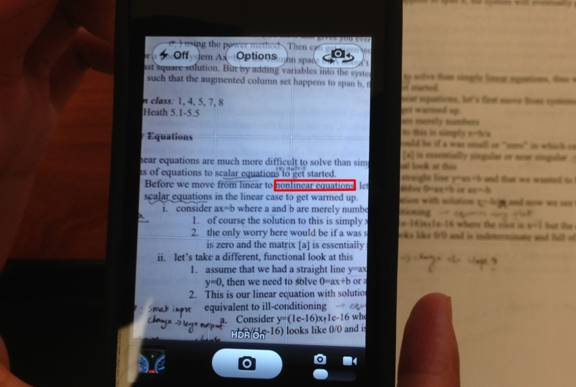
\includegraphics[scale=0.5]{demo.jpg}
\caption{Word Hunter Demo}
\end{figure}

\section{Preprocessing}
\subsection{Binarization}

The first step is to apply an adaptive thresholding algorithm in order to separate text from background in a grayscale image (which can be derived from RGB).  The reason we choose adaptive thresholding instead of global thresholding is that the lighting/brightness of the image is not uniform which will cause global thresholding to perform poorly in the extreme bright/dark regions.  We also observed that a blockSize of 41 yields the best thresholding result.  See Figure~\ref{noskew} and Figure~\ref{noskewbinarized} for an example of image before and after binarization.

\begin{figure}
\center
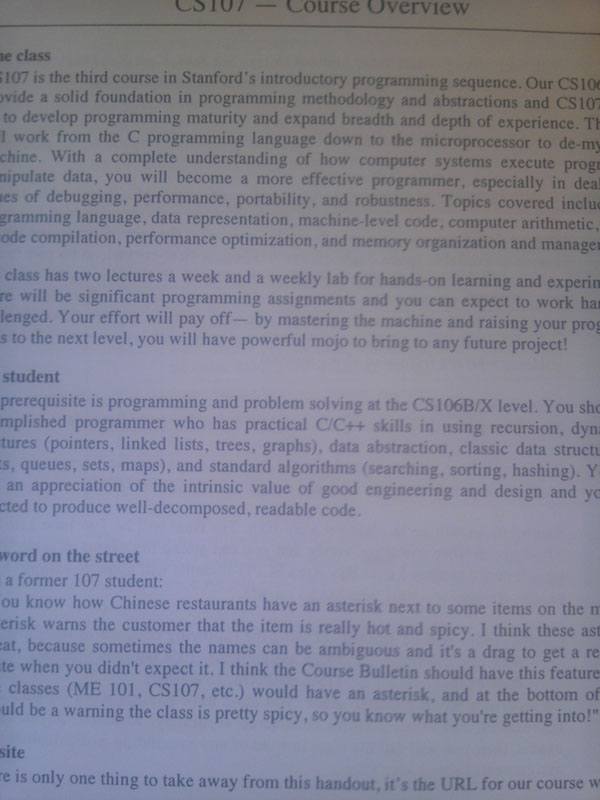
\includegraphics[scale=0.25]{no_skew.jpg}
\caption{Before Binarization}
\label{noskew}
\end{figure}

\begin{figure}
\center
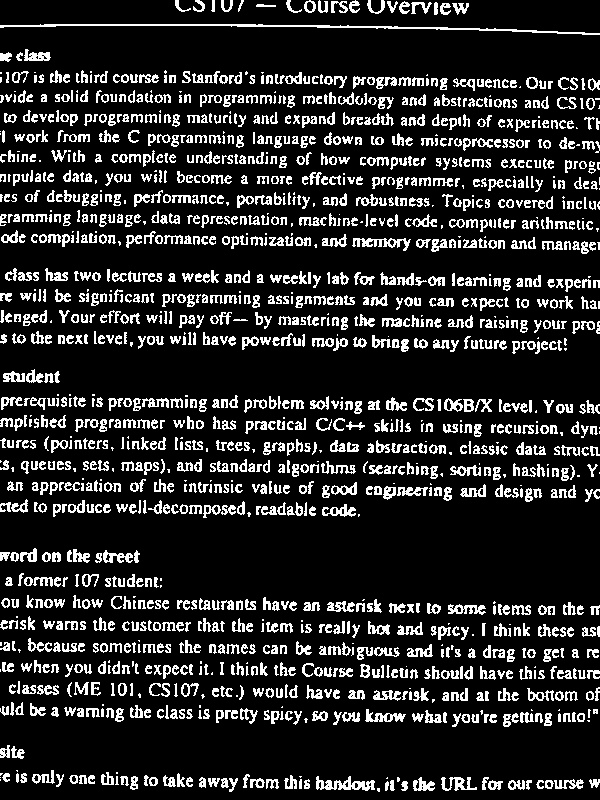
\includegraphics[scale=0.25]{no_skew_binarized.jpg}
\caption{After Binarization}
\label{noskewbinarized}
\end{figure}

\subsection{De-skew}

Hough transform is used to detect (text) lines in the image, we use OpenCV function HoughLinesP.  Then we rotate binarized image by the mean of the rotation angles calculated from each text line, we call OpenCV function getRotationMatrix2D to do it.  We also need to make sure not to cut off corners in the rotation process, therefore we need to pad the binarized image before rotating.  See Figure~\ref{binarized} and Figure~\ref{deskewed} for an example of image before and after de-skew.  Notice that Figure~\ref{deskewed} is slightly larger because of padding.

\begin{figure}
\center
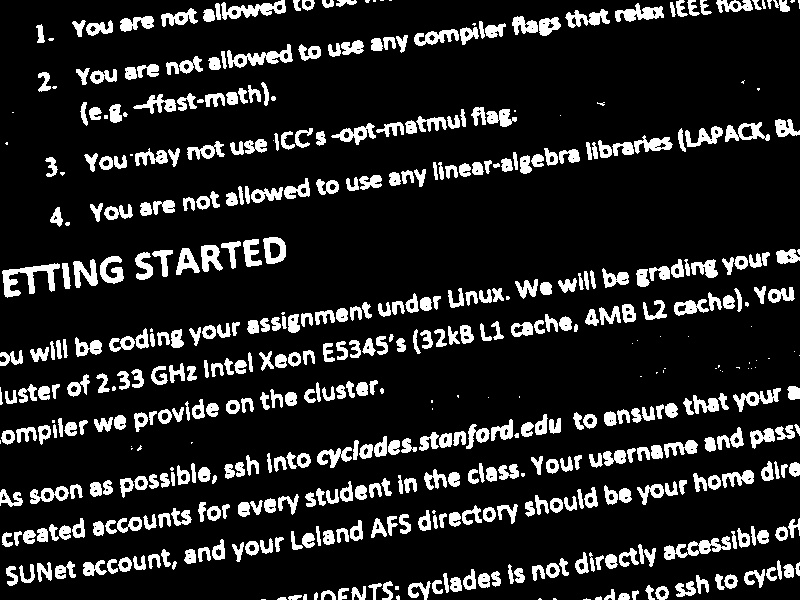
\includegraphics[scale=0.15]{binarized.jpg}
\caption{Binarized Image Before Deskew}
\label{binarized}
\end{figure}

\begin{figure}
\center
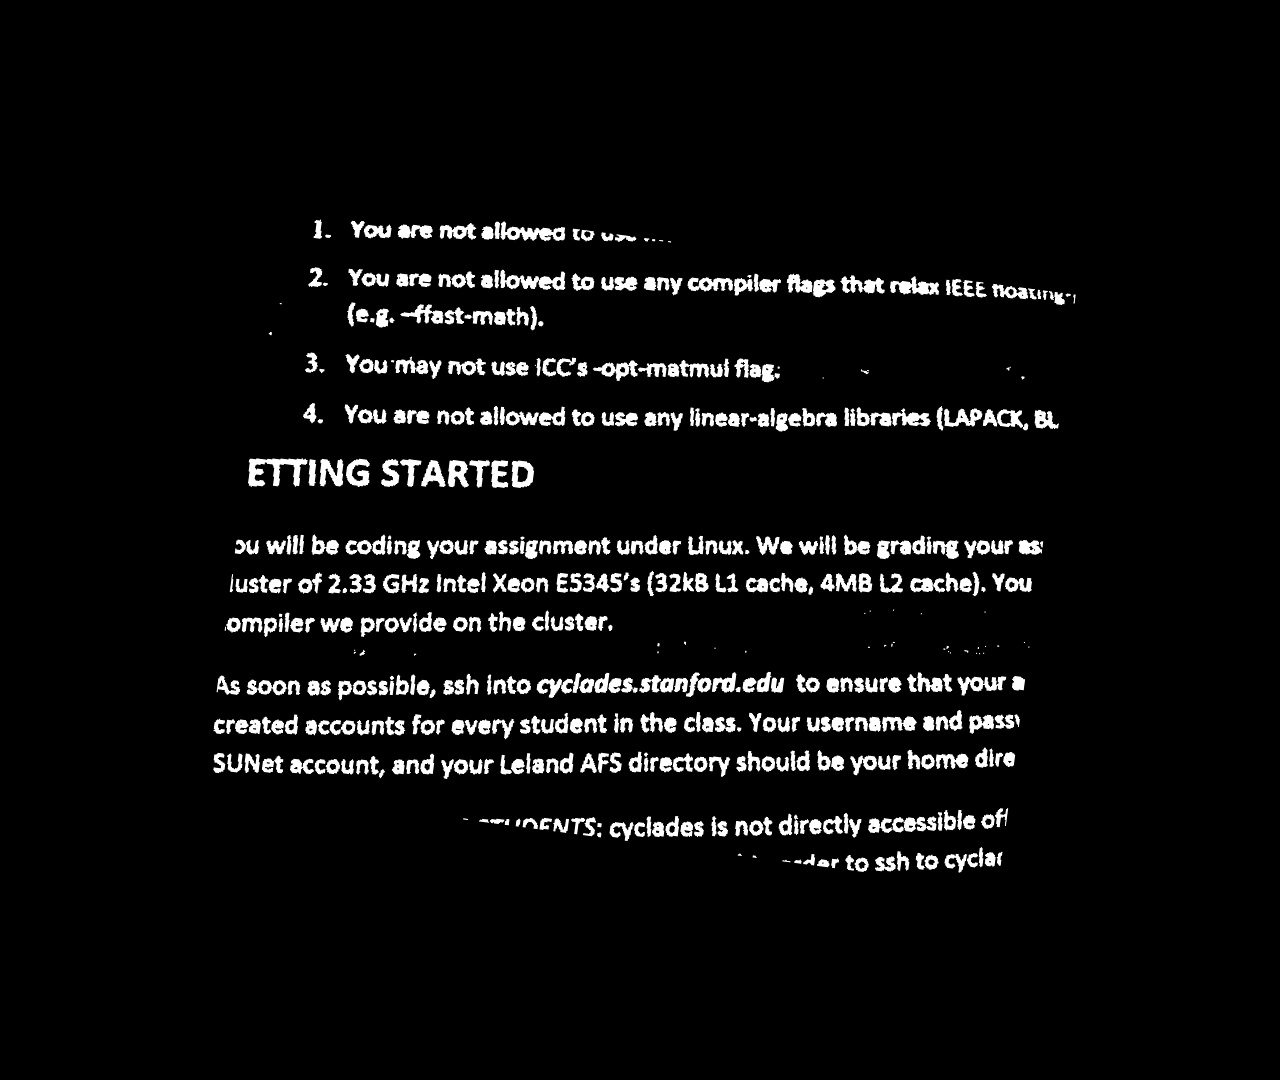
\includegraphics[scale=0.15]{deskewedImage.jpg}
\caption{Binarized And Deskewed}
\label{deskewed}
\end{figure}


\subsection{Layout analysis}

Find CharSize, Find Neighbour, FindDist.


\section{Word Recognition}

\section{Conclusion}

\section*{Acknowledgment}
We would like to thank David Chen and Sam Tsai for their generous and responsive help on the project.


%\begin{thebibliography}{1}
%\bibitem{IEEEhowto:kopka}
%H.~Kopka and P.~W. Daly, \emph{A Guide to \LaTeX}, 3rd~ed.\hskip 1em plus
%  0.5em minus 0.4em\relax Harlow, England: Addison-Wesley, 1999.
%\end{thebibliography}

\end{document}